\documentclass[a4paper,14pt]{extarticle} 
\usepackage[a4paper,top=1.5cm, bottom=1.5cm, left=2cm, right=1cm]{geometry}
%\usepackage[T2A]{fontenc}
%\usepackage[english, russian]{babel}
\usepackage{graphicx}
\graphicspath{{./pics/}}
\DeclareGraphicsExtensions{.pdf,.png,}
\usepackage[table]{xcolor}

\usepackage{fontspec}
\setmainfont{Times New Roman}
\setsansfont{FreeSans}
\setmonofont{FreeMono}
\renewcommand{\baselinestretch}{1.5}
\usepackage{polyglossia}
\setdefaultlanguage{russian}
\setotherlanguages{english,russian}
\usepackage{setspace}
\usepackage[many]{tcolorbox}
\usepackage{array}
\usepackage{longtable}

\begin{document}
    \begin{center}
        \thispagestyle{empty}
        \begin{singlespace}
        ФЕДЕРАЛЬНОЕ АГЕНТСТВО СВЯЗИ

        ФЕДЕРАЛЬНОЕ ГОСУДАРСТВЕННОЕ БЮДЖЕТНОЕ ОБРАЗОВАТЕЛЬНОЕ

        УЧРЕЖДЕНИЕ ВЫСШЕГО ОБРАЗОВАНИЯ

        «САНКТ-ПЕТЕРБУРГСКИЙ ГОСУДАРСТВЕННЫЙ УНИВЕРСИТЕТ ТЕЛЕКОММУНИКАЦИЙ ИМ. ПРОФ. М.А. БОНЧ-БРУЕВИЧА»

        (СПбГУТ)
        \end{singlespace}
        \vspace{-1ex}
        \rule{\textwidth}{0.4pt}
        \vspace{-5ex}

        \vspace{100px}
        \textbf{Лабораторная работа №4}\\
        Исследование свойств модели резисторного каскада с общей базой в частотной и временной областях на ПК

    \vspace{100px}
    \end{center}
    \vspace{4ex}
    \begin{flushright}
    \parbox{12 cm}{
    \begin{flushleft}
        Выполнила бригада:\\
        Группа ИКТЗ-83\\
        \underline{Громов А.А., Миколаени М.С., Мазеин Д.С.} \hfill \rule[-0.85ex]{0.09\textwidth}{0.6pt}\\
        \vspace{-1ex}
        \footnotesize \textit{ (Ф.И.О., № группы) \hfill (подпись)} \normalsize


    \end{flushleft}
    }
    \end{flushright}
    \begin{center}
        \vfill
        Санкт-Петербург

        2020

    \end{center}
    \newpage

    \textbf{Цель работы:} Изучить свойства усилительного каскада с общим коллектором (ОК) в режиме малого сигнала. Выполнить анализ в частотной и временной областях. Исследовать свойства каскада при изменении сопротивлений источника сигнала, нагрузки и элементов схемы. Определить входное и выходное сопротивления каскада.

    % \textbf{\emph{Объектом исследования}} является схема усилительного каскада на
    % биполярном транзисторе с общим коллектором. По определению в схеме с ОК
    % коллектор транзистора присоединяется к проводу, общему для входа и выхода
    % каскада. На рис. 1, а показано простейшее изображение схемы с ОК.
    
    % \begin{center}
    %     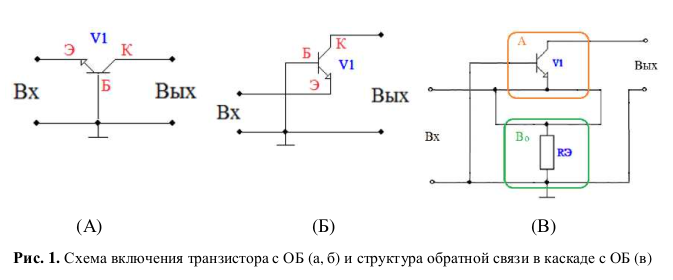
\includegraphics[scale=0.85]{0.1.png}
    % \end{center}

    % Другое представление транзистора с ОК показано на рис. 1, б. Такое
    % изображение каскада с ОК позволяет рассматривать его как структуру с ОЭ,
    % охваченную ОС. В этой схеме имеет место последовательная по входу и
    % параллельная по выходу отрицательная ОС (рис. 1, в). Полная принципиальная
    % схема каскада ОК представлена на рис. 2)

    % \begin{center}
    %     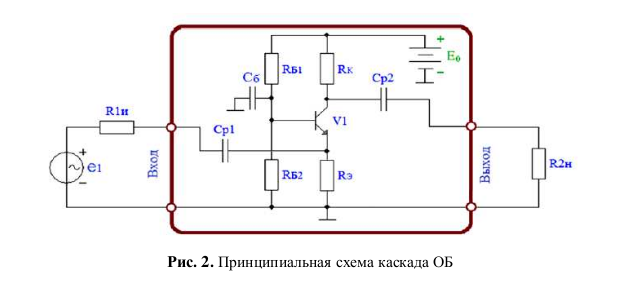
\includegraphics[scale=0.85]{0.2.png}
    % \end{center}

    % Переменная составляющая сигнала поступает на базу транзистора через
    % разделительный конденсатор $C_{\text{Р1}}$ , а передается в нагрузку $R_{2H}$ через
    % разделительный конденсатор $C_{P2}$ из эмиттера. Сопротивление источника
    % питания $E_0$ переменному току практически равно нулю, поэтому коллектор
    % оказывается соединенным с общим проводом и схема соответствует структуре
    % соединений на рис. 1, б. В схеме с ОК, как правило, не включают в
    % коллекторную цепь резистор $R_K$ . В этом случае всё напряжение питания
    % делится между транзистором и $R_{\text{Э}}$ . При питании транзистора с эмиттерной
    % стабилизацией, применённой здесь, ток покоя изменяется незначительно, а
    % увеличение напряжений между электродами транзистора ($U_{\text{КЭ}}$ и особенно $U_{\text{КБ}}$)
    % снижает значение ёмкости $C_K$ . Этот факт и отсутствие эффекта Миллера (при
    % $R_K$ = 0)дают основания для сохранения модели транзистора неизменной.

    % В работе используются данные лабораторного макета, при этом
    % сохраняются номинальные значения всех элементов схемы, напряжение
    % питания, ток покоя, транзистор КТ503В, согласно рис.2.1 [1]. В этой работе
    % моделируется усилитель на основе реального действующего макета.
    % Эквивалентная схема усилителя с ОК для переменного тока изображена на
    % рис. 3. Входной сигнал поступает через разделительный конденсатор $C_{\text{Р1}}$ на
    % базу транзистора (узел 2). Элемент $R_{\text{б}}$ отражает эквивалентное сопротивление
    % базового делителя – параллельное включение $R_{\text{б1}}$ и $R_{\text{б2}}$ . Выходной сигнал через
    % разделительный конденсатор $C_{Р2}$ подаётся в нагрузку $R_{\text{2н}}$, $C_{\text{2н}}$ (узел 7)
    % Коллектор транзистора заземлён непосредственно и является общим для входа
    % и выхода усилителя. Другие элементы эквивалентной схемы соответствуют
    % приведённым на рис. 3 и соответствуют параметрам лабораторного макета.
    % Значения внутренних ёмкостей транзистора и его средний коэффициент
    % усиления тока $h_{21}$ взяты из справочных данных. В схему введено выходное
    % сопротивление транзистора 1/ $h_{22}$ . Оно определяется током покоя $I_{0K}$ = 4 мА и
    % ориентировочным значением напряжения Эрли, равным 100 В. При токе
    % коллектора $I_{0K}$ = 4 мА и $h_{21}$ = 75 в базе транзистора протекает ток $I_{\text{0Б}}$ = 53 мкА.
    % Принимая $U_T$ = 25.6 мВ, получаем сопротивление перехода база-эмиттер
    % rбэ = 470 Ом.

    % \begin{center}
    %     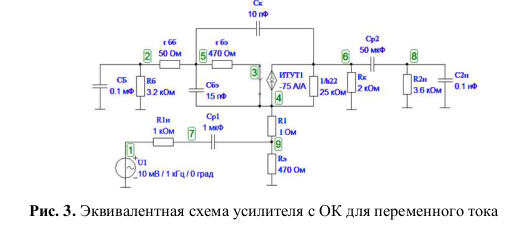
\includegraphics[scale=0.9]{0.3.png}
    % \end{center}

    \newpage
    \textbf{Пункт 1:}
    \begin{center}
        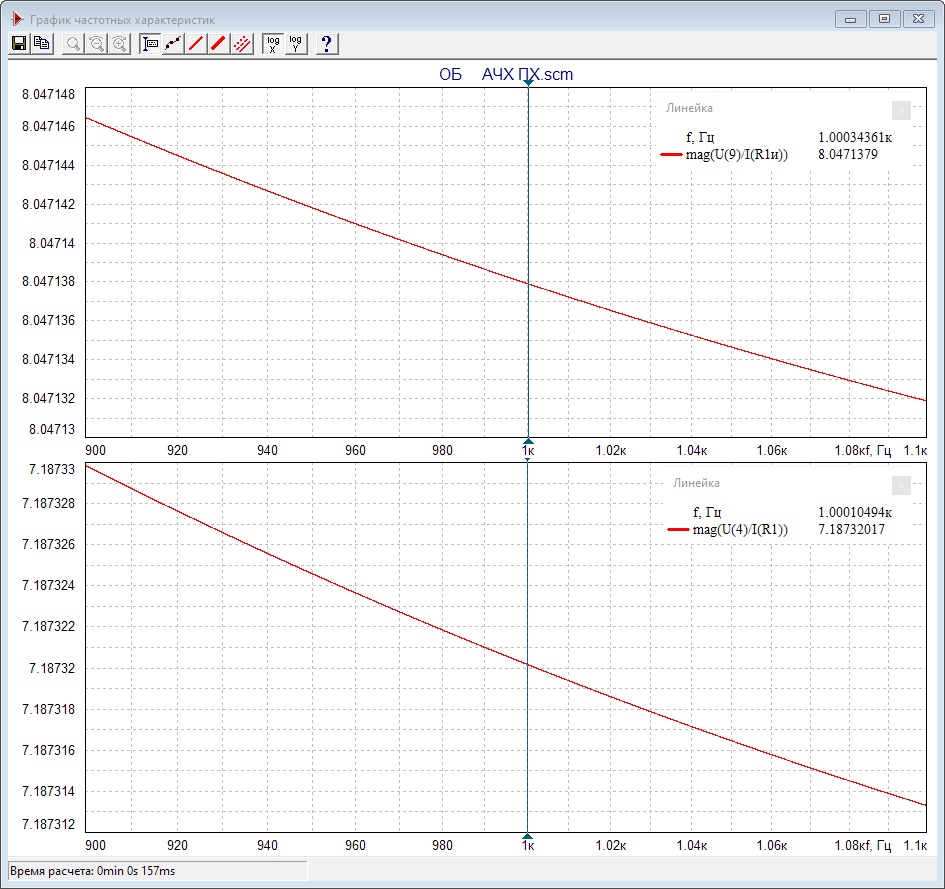
\includegraphics[scale=0.3]{1.png}
    \end{center}
    \begin{center}
        Входное сопротивление с учетом и без учета резистора $R_{\text{э}}$ 
    \end{center}
    \begin{table}[ht]
        \begin{center}
            \caption{Измерение входного сопротивления каскада с ОБ}
            \begin{tabular}{ |c|c| }
                \hline
                Измерение & Величина входного сопротивления\\
                \hline
                с учётом сопротивления $R_{\text{э}}$ & 8,04 Ом\\
                \hline
                без учёта сопротивления $R_{\text{э}}$ & 7,18 Ом\\
                \hline
            \end{tabular}
        \end{center}
    \end{table}
    \textbf{Выводы по пункту 1:}
    \vspace{-6ex}
    \begin{singlespace}
        \begin{itemize}
            \item Входное сопротивление каскада с ОБ с учетом сопротивления $R_{\text{э}}$ примерно на 3 порядка меньше,
             чем входное сопротивление каскада с ОК с учетом сопротивления $R_{\text{б}}$.
            \item Входное сопротивление каскада с ОБ без учета сопротивления $R_{\text{э}}$ примерно на 3 порядка меньше,
             чем входное сопротивление каскада с ОК без учета сопротивления $R_{\text{б}}$.
        \end{itemize}
    \end{singlespace}


    \newpage
    \textbf{Пункт 2:}
    \begin{center}
        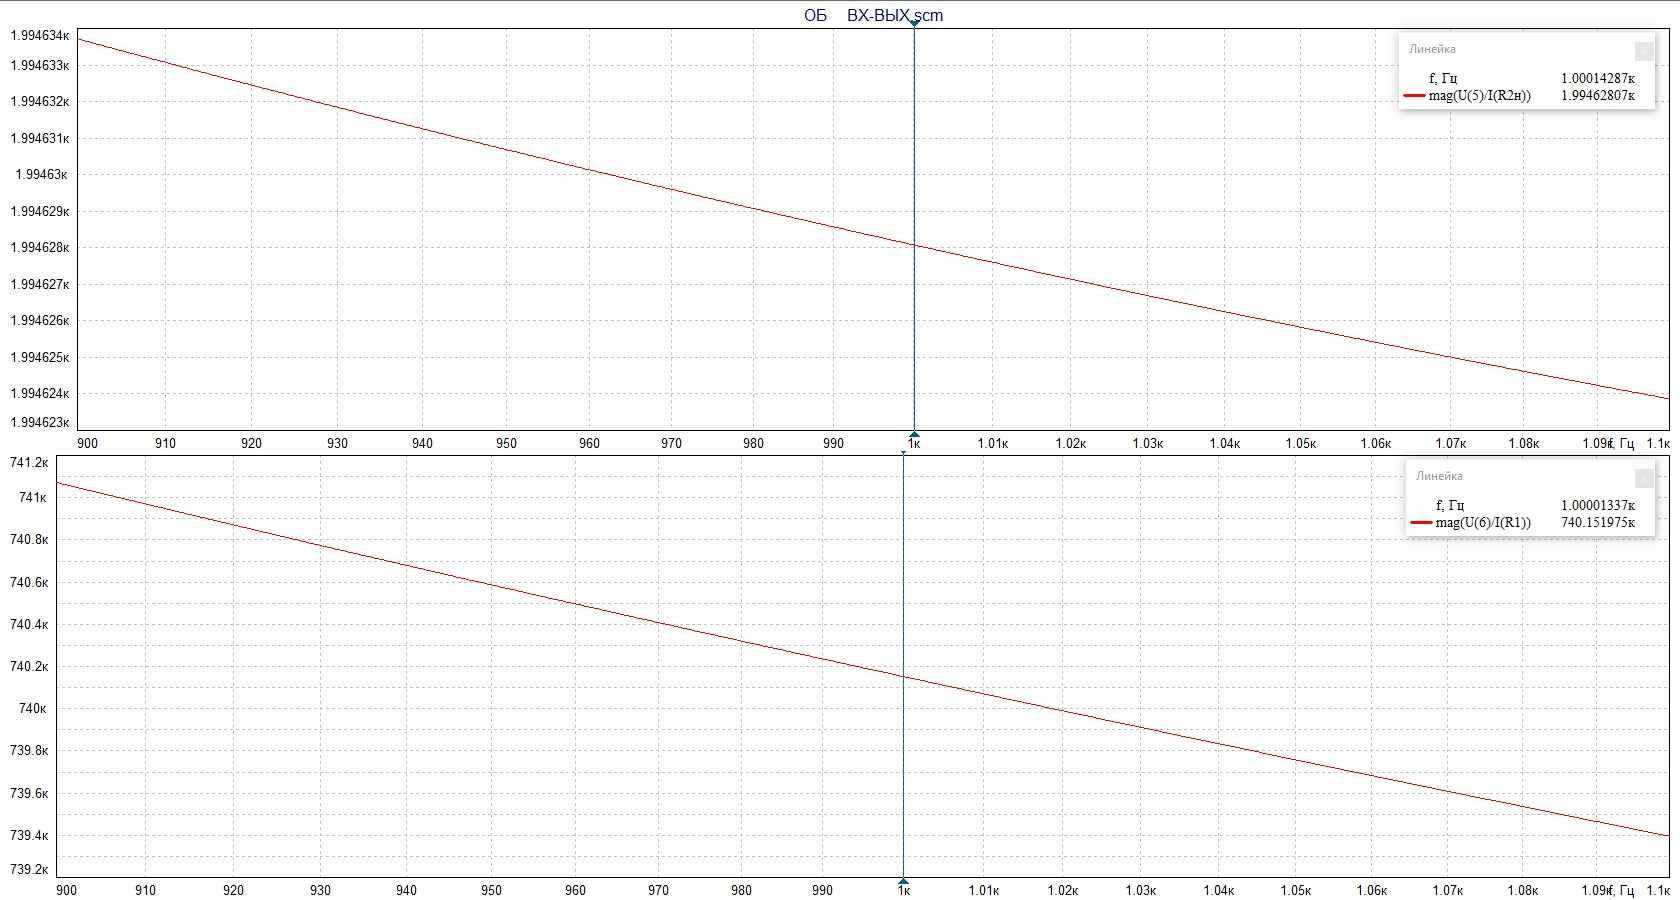
\includegraphics[scale=0.25]{2.jpg}
    \end{center}
    \begin{center}
        Выходное сопротивление транзистора и каскада
    \end{center}
    \begin{table}[ht]
        \begin{center}
            \caption{Измерение выходного сопротивления каскада с ОБ}
            \begin{tabular}{ |c|c| }
                \hline
                Измерение & Величина выходного сопротивления
                \tabularnewline
                \hline
                с учетом сопротивления $R_{\text{э}}$ & 1,994 кОм
                \tabularnewline
                \hline
                без учета сопротивления $R_{\text{э}}$ & 740,15 кОм
                \tabularnewline
                \hline
            \end{tabular}
        \end{center}
    \end{table}

    \textbf{Выводы по пункту 2:}
    \vspace{-6ex}
    \begin{singlespace}
        \begin{itemize}
            \item Выходное сопротивление каскада с ОБ примерно на 3 порядка больше, 
            чем выходное сопротивление касакада с ОК.
            
        \end{itemize}
    \end{singlespace}

    \newpage 
    \textbf{Пункт 3:}
    \begin{center}
        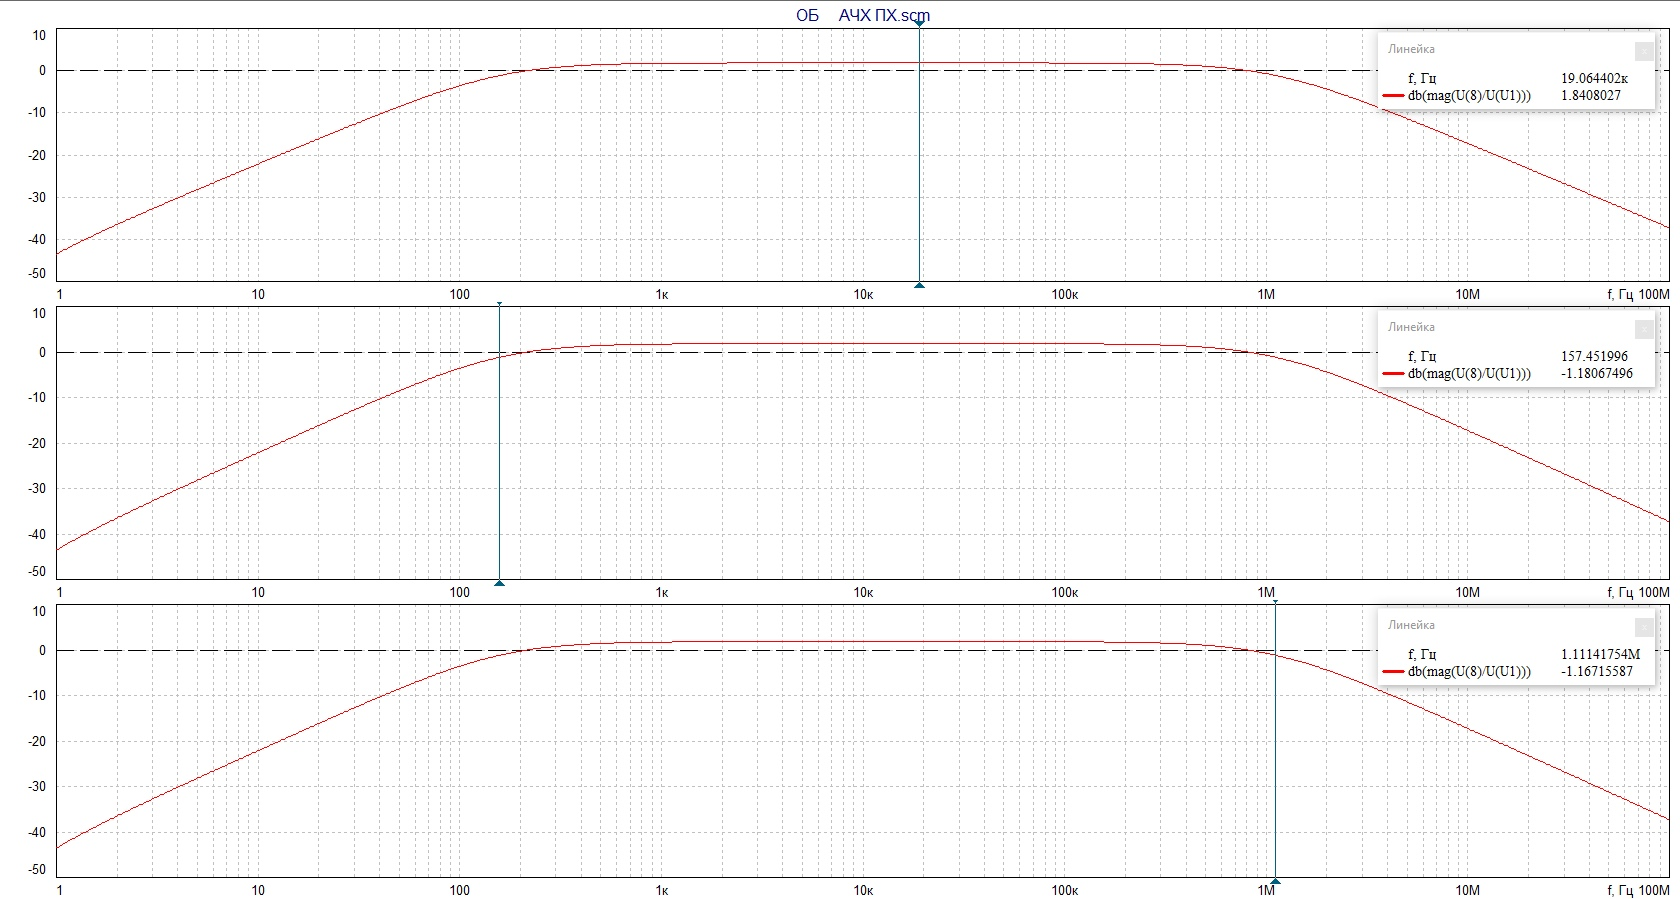
\includegraphics[scale=0.25]{3.jpg}
    \end{center}
   \begin{center}
        АЧХ и ФЧХ каскада
    \end{center}

    \begin{table}[ht]
        \begin{center}
            \caption{Измерение АЧХ каскада с ОБ}
            \begin{tabular}{ |c|c|c|c|c| }
                \hline
                $K_{\text{скв}}$, Дб & ($K_{\text{скв}}$ - 3), Дб&fн, Гц & fв, МГц & ∆f=fв−fн, МГц \\
                \hline 
                1.84 & -1.16 & 157.45 & 1,11 & 1.1098 \\
                \hline
            \end{tabular}\\
        \end{center}
    \end{table}
    \vspace{-1cm}
    $K_{\text{ОБскв}}=\frac{R_{\text{Э}}}{R_{\text{1И}}+R_{\text{Э}}}\cdot\frac{h_{21}R_{\text{Н}}}{h_{11}+R_{\text{Г}}(1+h_{21})}$
    \begin{center}
        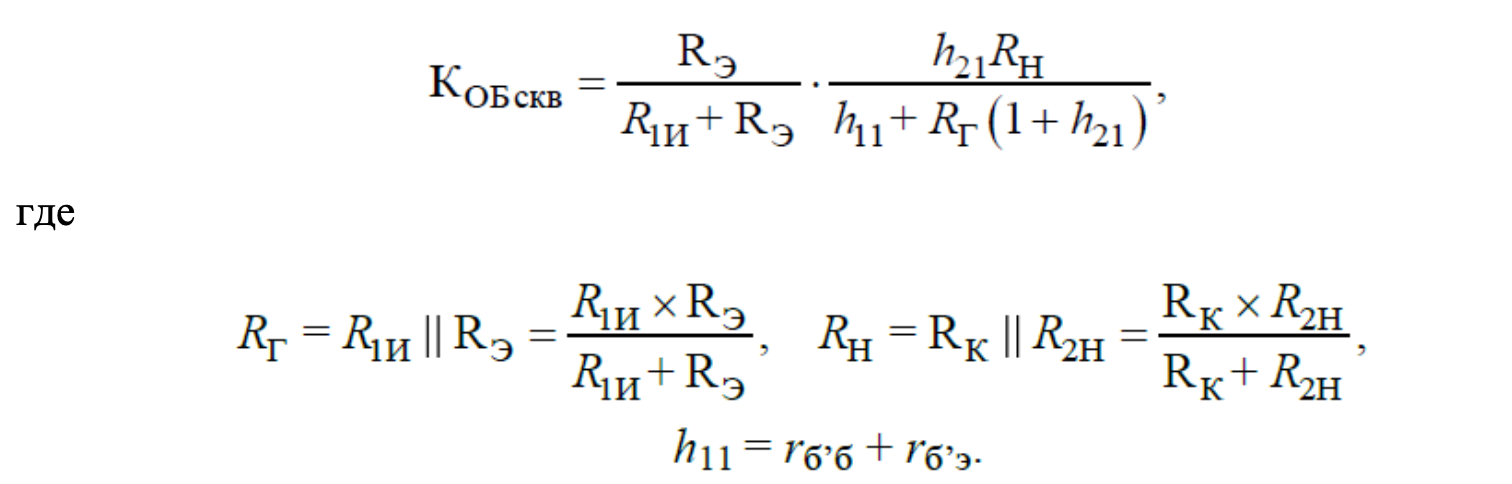
\includegraphics[scale=0.45]{form.png}
    \end{center}
    \begin{center}
        $K_{\text{ОБскв}}=\frac{75\cdot(\frac{2000\cdot36000}{2000+3600})}{520+(\frac{1000\cdot470}{1470})\cdot1+75)} = 1.24 = 1.87\text{Дб}$
    \end{center}

    \textbf{Выводы по пункту 3:}
    \vspace{-6ex}
    \begin{singlespace}
        \begin{itemize}
            \item Схема каскада с ОБ усиливает сигнал, в отличие от схемы с ОК.
            \item Рабочая полоса частот у схемы каскада с ОБ значительно меньше, чем у схемы с ОК.
            \item Экспериментальный коэффициент сквозного усиления практически совпадает с теоретическим.
        \end{itemize}
    \end{singlespace}


    \newpage
    \textbf{Пункт 4:}
    \vspace{-1cm}
    \begin{table}[h!]
        \small
        \begin{center}
            \caption{Измерение ПХ каскада с ОК}
            \begin{tabular}{|>{\centering}m{7.6cm}|>{\centering}m{8.5cm}|}
                \hline 
                \rowcolor{gray} Время импульса & $t_{\text{и}}$= 25 мкс 
                \tabularnewline
                \hline
                Частота f, Гц & 20000
                \tabularnewline
                \hline 
                Осциллограмма импульса & \begin{center}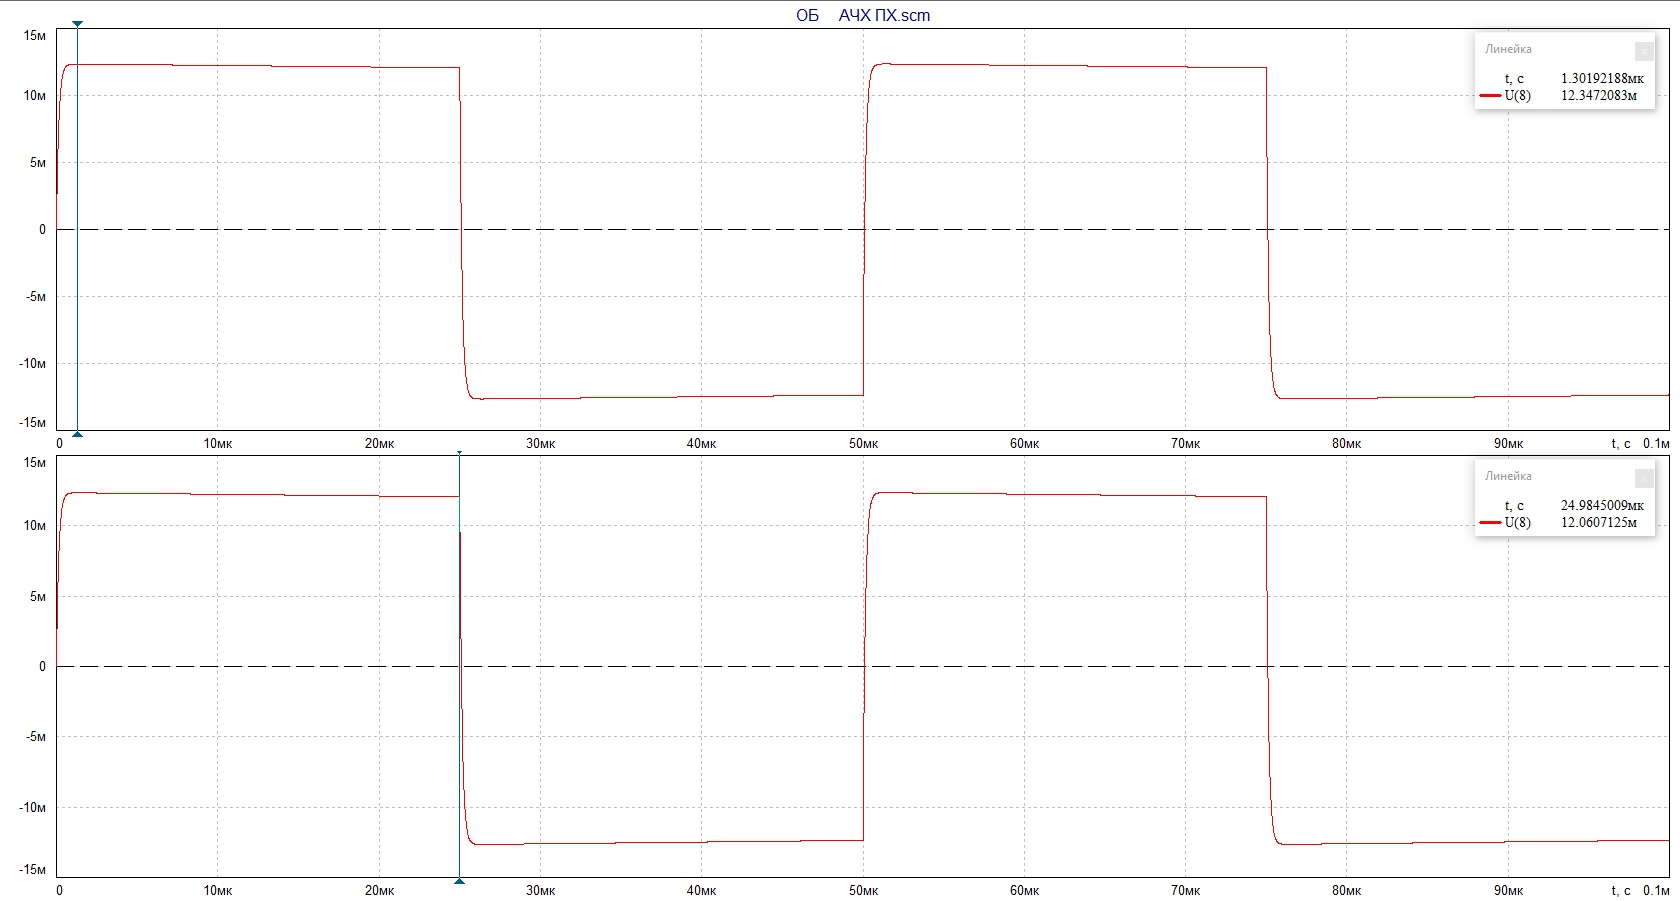
\includegraphics[scale=0.08]{4.1.jpg}\end{center}
                \tabularnewline
                \hline 
                \parbox[c][3cm]{7.6cm}{
                    Измеренный спад вершины импульса ∆, \% 
                    \begin{center}
                        $∆=\frac{U_{\text{уст}}-U_{\text{вых}}}{U_{\text{уст}}} \cdot 100\%$
                    \end{center} 
                    }& 2.35
                \tabularnewline
                \hline 
                Рассчитанный спад вершины импульса ∆, \% & 2.47 
                \tabularnewline
                \hline 
                \multicolumn{2}{|c|}{Осциллограмма увеличенной области нарастания импульса} 
                \tabularnewline
                \hline 
                \multicolumn{2}{|c|}{\parbox[c]{5cm}{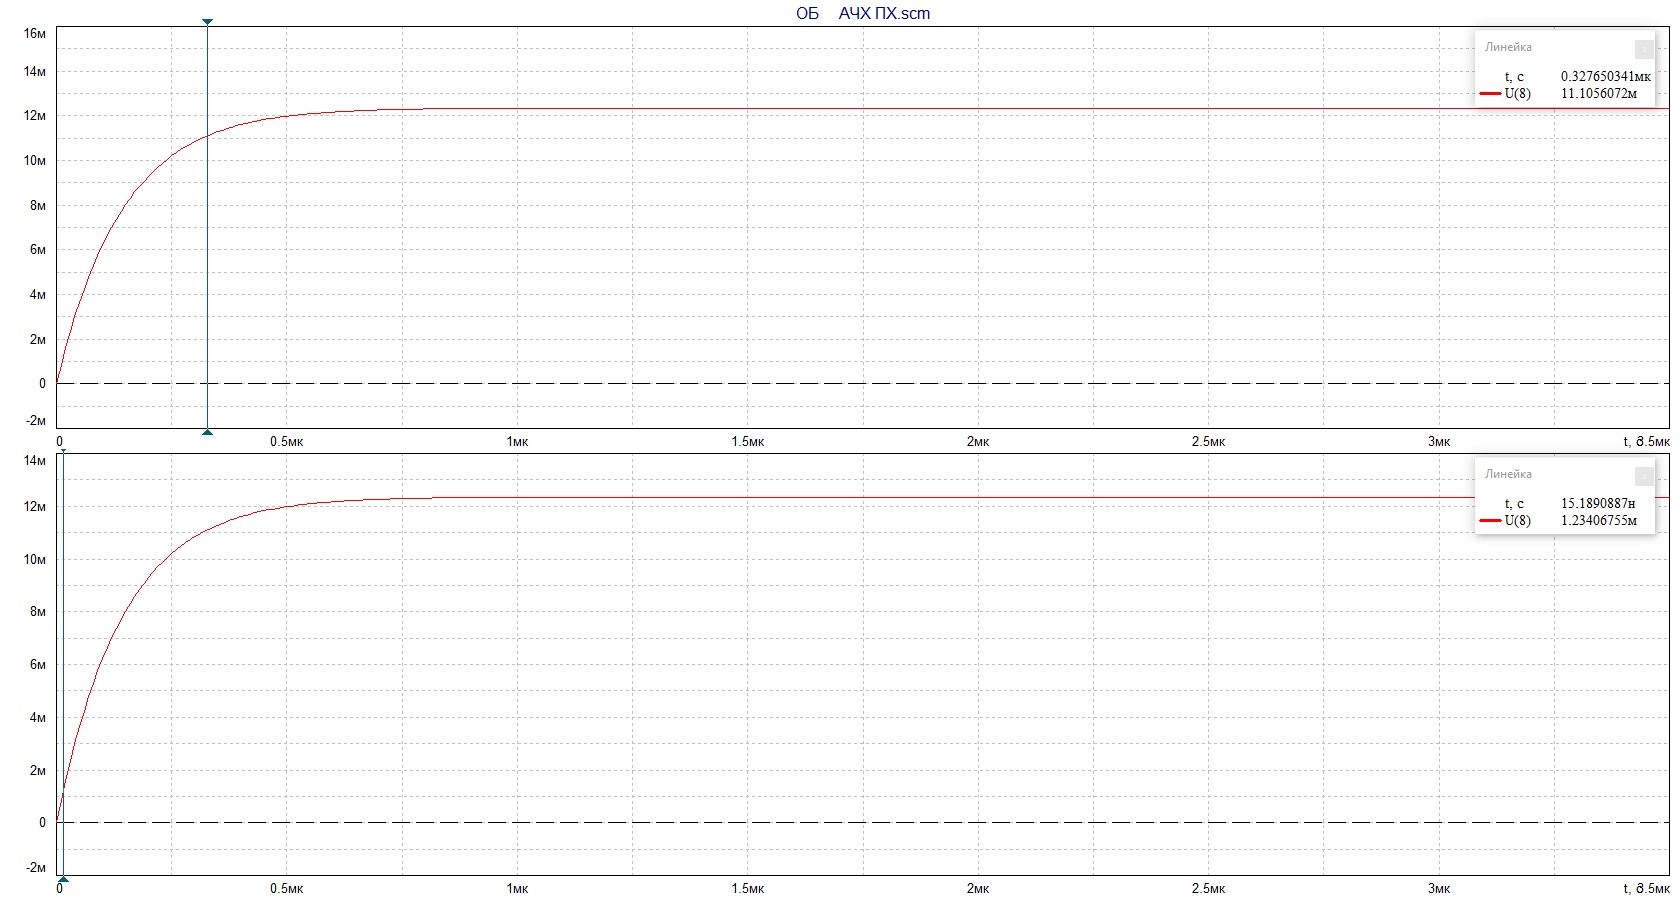
\includegraphics[scale=0.08]{4.2.jpg}}}
                \tabularnewline
                \hline
                \parbox[c][3cm]{7.6cm}{Измеренное время нарастания импульса \\ $t_{\text{Н}}$ = $t_{\text{2}}$ – $t_{\text{1}}$, нс} & 312.8
                \tabularnewline
                \hline 
                Рассчитанное время нарастания импульса $t_{\text{н}}$, нс & 315.3
                \tabularnewline
                \hline 
           \end{tabular}
        \end{center}
    \end{table}

    \vspace{-1.2cm}
    \begin{table}[h!]
        \small
        \begin{center}
            \begin{tabular}{|>{\centering}m{7.6cm}|>{\centering}m{8.5cm}|}
                \hline
                \rowcolor{gray} Время импульса & $t_{\text{и}}$= 1.25 мс 
                \tabularnewline
                \hline
                Частота f, Гц & 400
                \tabularnewline
                \hline 
                \multicolumn{2}{|c|}{Осциллограмма импульса}
                \tabularnewline
                \hline
                \multicolumn{2}{|c|}{\parbox[c]{6cm}{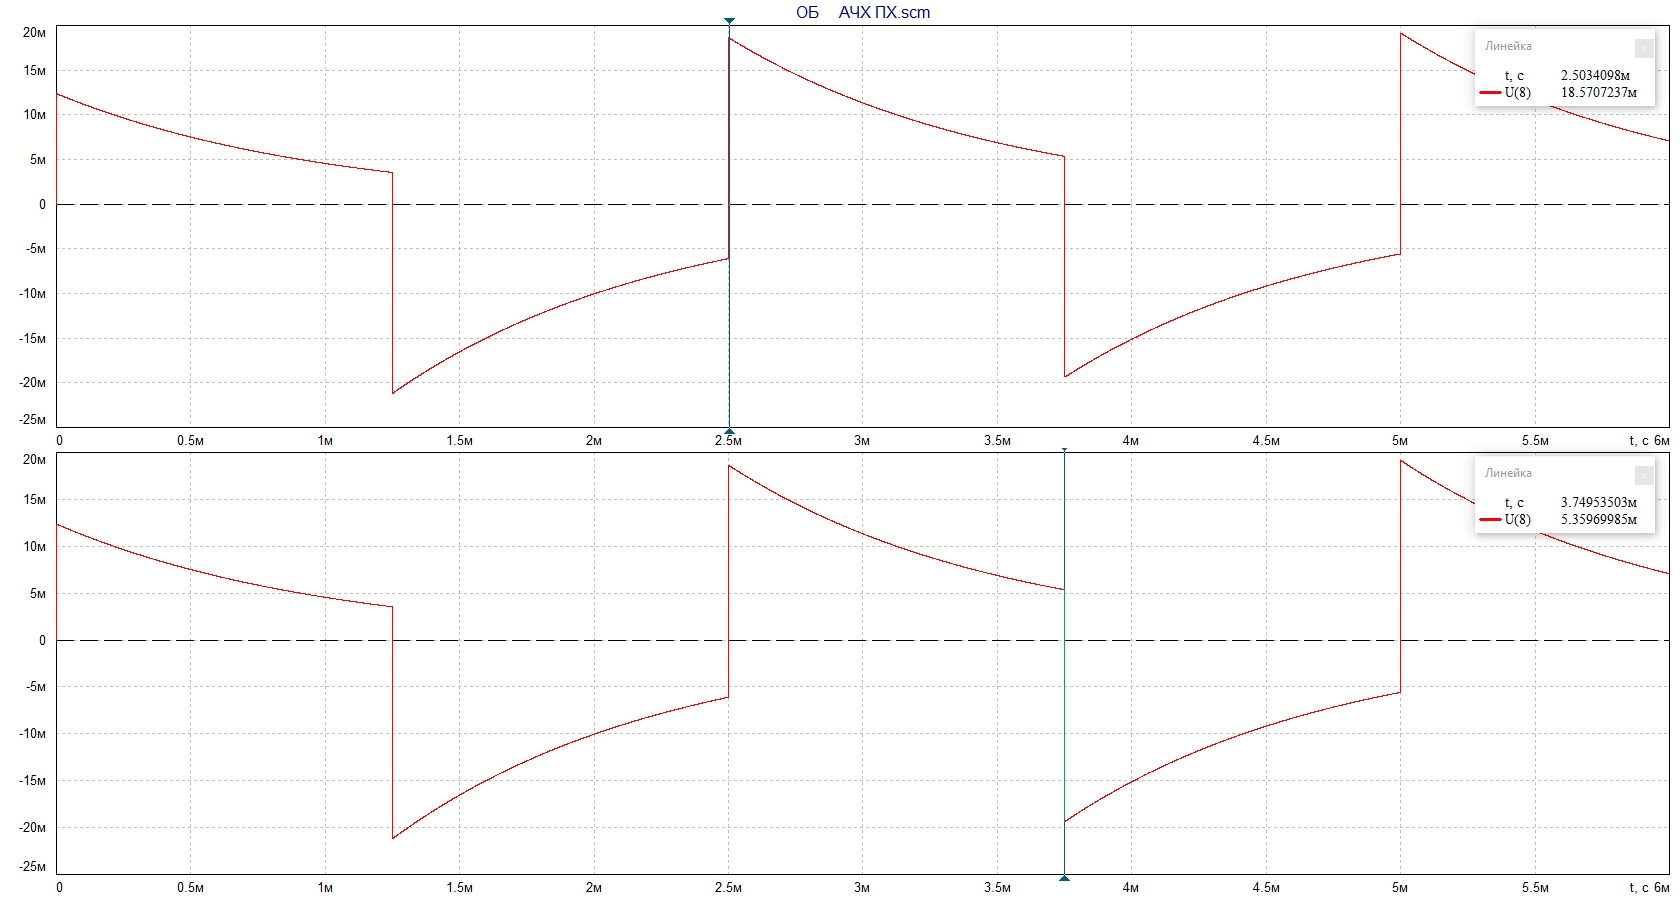
\includegraphics[scale=0.08]{4.3.jpg}}}
                \tabularnewline
                \hline
                \parbox[c][2cm]{7.6cm}{
                    Измеренный спад вершины импульса ∆, \% 
                    \begin{center}
                        $∆=\frac{U_{\text{уст}}-U_{\text{вых}}}{U_{\text{уст}}} \cdot 100\%$
                    \end{center} 
                    }& 71
                \tabularnewline
                \hline 
                Рассчитанный спад вершины импульса ∆, \% & 124
                \tabularnewline
                \hline
            \end{tabular}
        \end{center}
    \end{table}

    \newpage
    \textbf{Выводы по пункту 4:}
    \vspace{-4ex}
    \begin{singlespace}
        \begin{itemize}
            \item Измеренный спад вершины импульса практически совпадает с рассчитанным спадом вершины импульса при $t_\text{и}=25\text{мкс}$;
            \item Измеренное время нарастания импульса практически совпадает с рассчитанное временем нарастания импульса при $t_\text{и}=25\text{мкс}$;
            \item Расхождение рассчитанного и измеренного спада импульса объясняется тем, что при частоте 400Гц измерения происходят в нелинейной зоне АЧХ. Избежать этого можно, изменив значение Cр1 и тогда рассчитанный спад вершины импульса будет совпадать с измеренным (например при Cр1=12мкФ, частота нижнего среза = 13,2Гц, ∆рас = 10,4\%, ∆изм = 10,2\%)  
        \end{itemize}
    \end{singlespace}

    \textbf{Пункт 5}
    \begin{table}[ht]
        \begin{center}
            \caption{Оценка влияния параметров схемы на ПХ и АЧХ}
            \begin{tabular}{|c|c|c|c|c|c|c|c|}
                \hline 
                № & $R_1$ & $R_2$ & $K_{\text{скв}}$ & $f_{\text{н}}$ & $f_{\text{в}}$ & \parbox[c]{4cm}{\begin{center}∆ \\при $t_{\text{и}}$= 25 мкс \end{center}} & \parbox[c]{4cm}{\begin{center}$t_{n}$ \\при $t_{\text{и}}$= 1.25 мс \end{center}}
                \tabularnewline
                \hline 
                п/п & кОм & кОм & дБ & Гц & МГц & \% & нс
                \tabularnewline
                \hline 
                1 & 1 & 3.6	& 1.84 & 0.16 & 1.11 & 71.20 & 310
                \tabularnewline
                \hline 
                2 & 1 & 10 & 4.09 & 0.16 & 0.86 & 71.10 & 402
                \tabularnewline
                \hline        
                3 & 0.1 & 3.6 & 21.228 & 1.47 & 1.07 & 99.56 & 310
                \tabularnewline
                \hline        
                4 & 0.1 & 10 & 23.466 & 1.46 & 0.84 & 99.66 & 390
                \tabularnewline
                \hline        
            \end{tabular}
        \end{center}
    \end{table}

    \begin{center}
        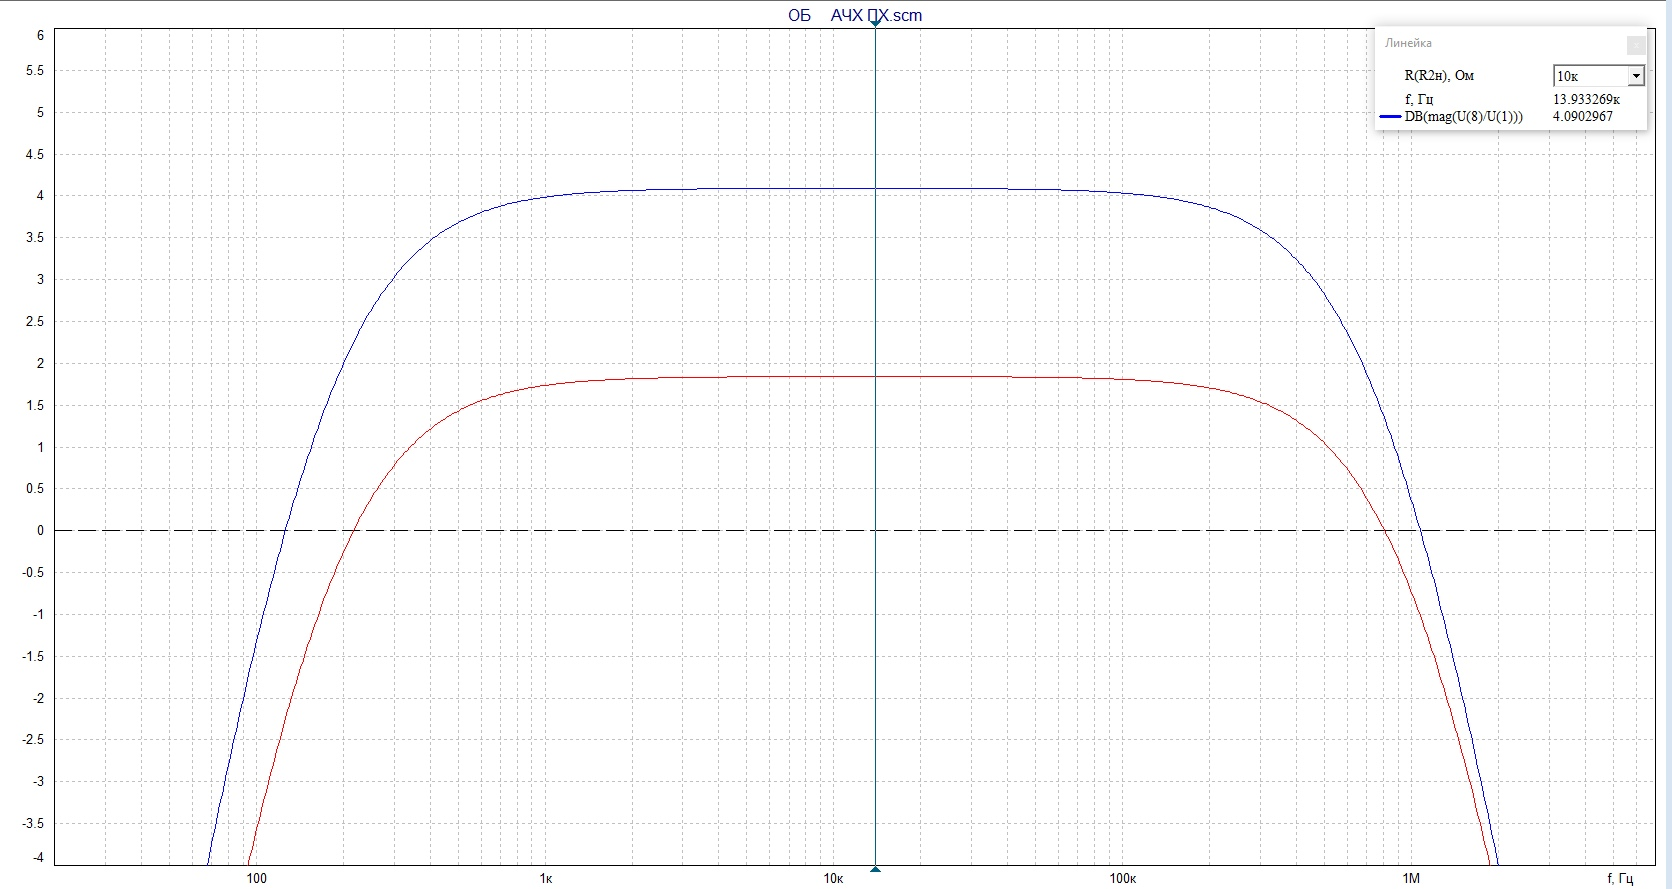
\includegraphics[scale=0.3]{5.1.jpg}
    \end{center}

    АЧХ при $R_1$ = 1000 Ом

     \begin{center}
         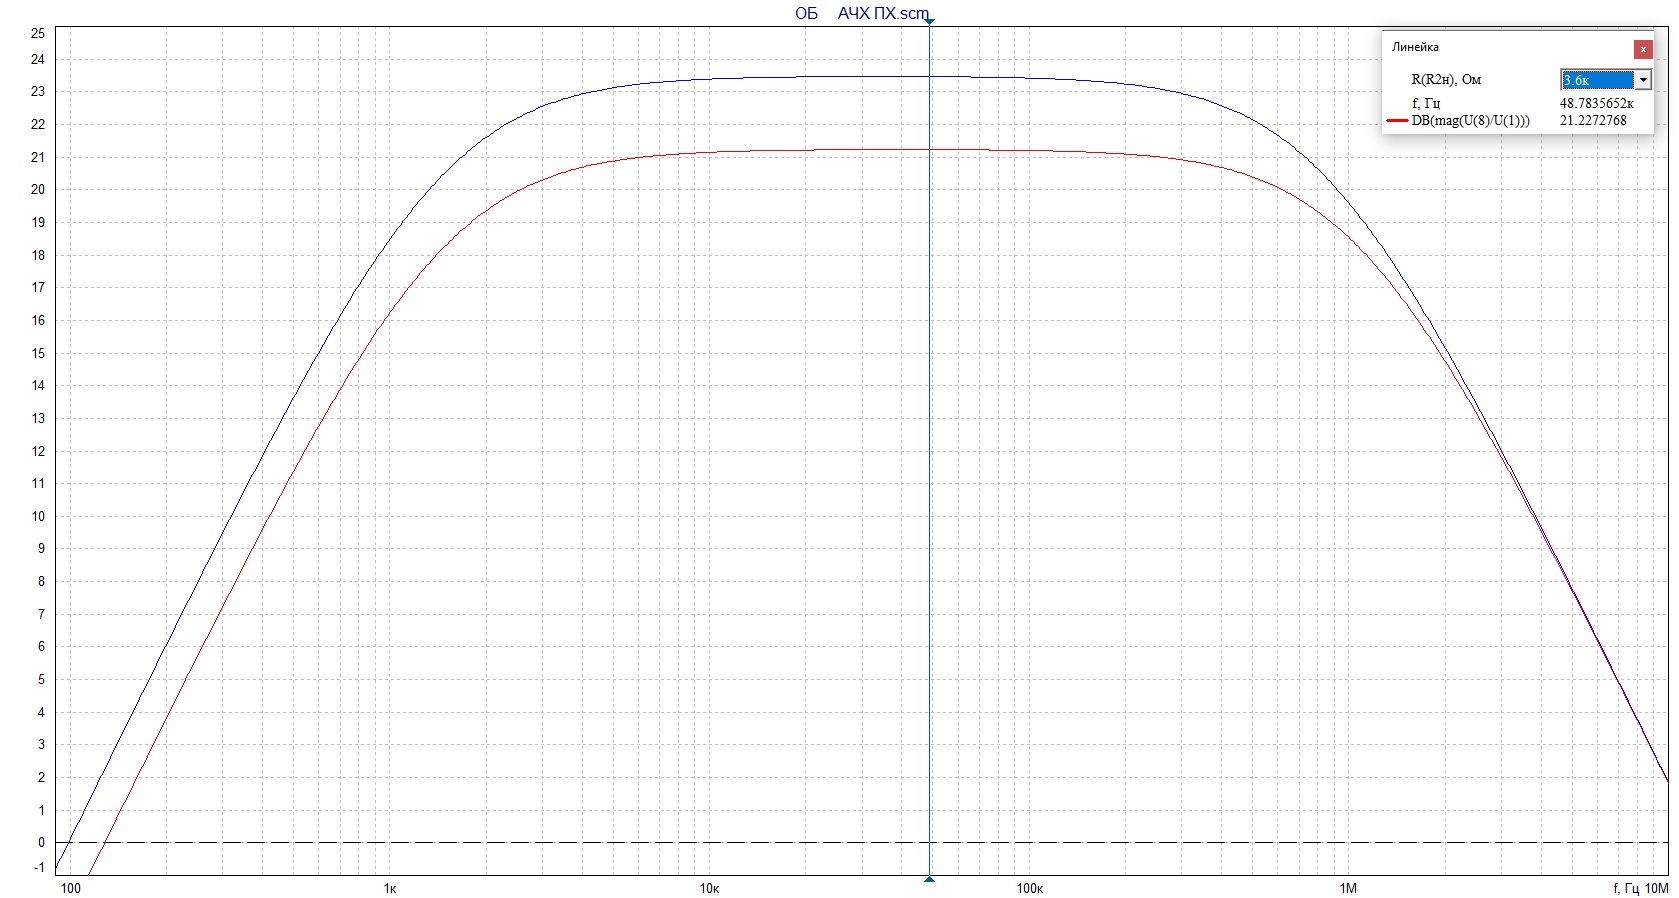
\includegraphics[scale=0.3]{5.2.jpg}
     \end{center}

    АЧХ при $R_1$ = 100 Ом

    \begin{center}
        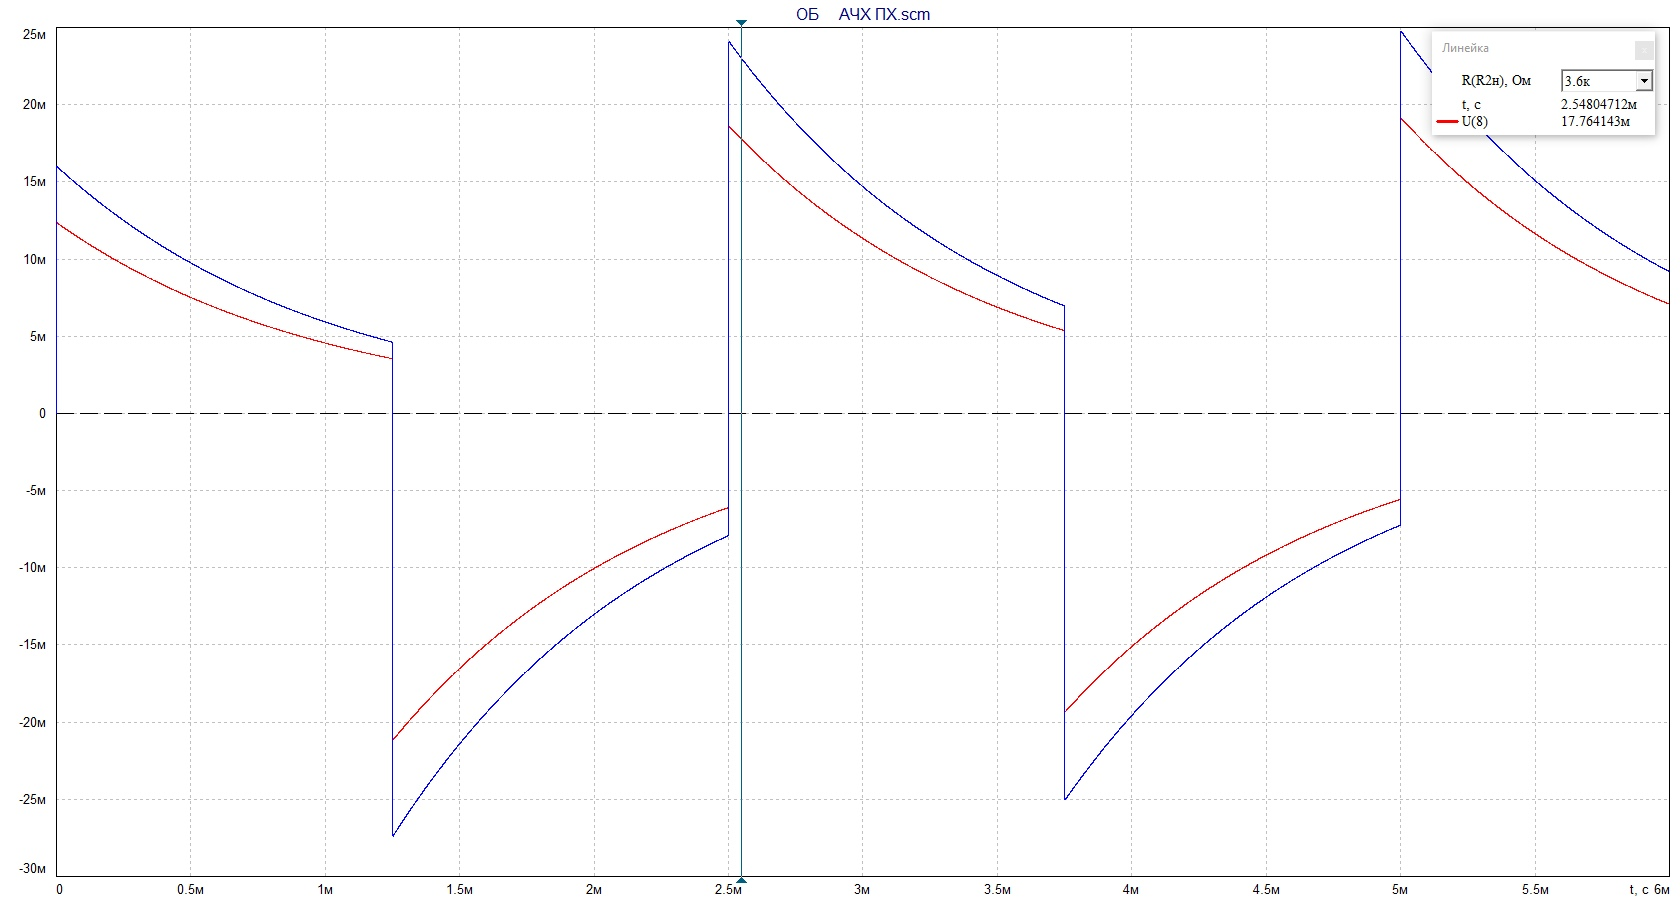
\includegraphics[scale=0.3]{5.3.jpg}
    \end{center}

    ПХ при $R_1$ = 1000 Ом, f = 400 Гц

    \begin{center}
        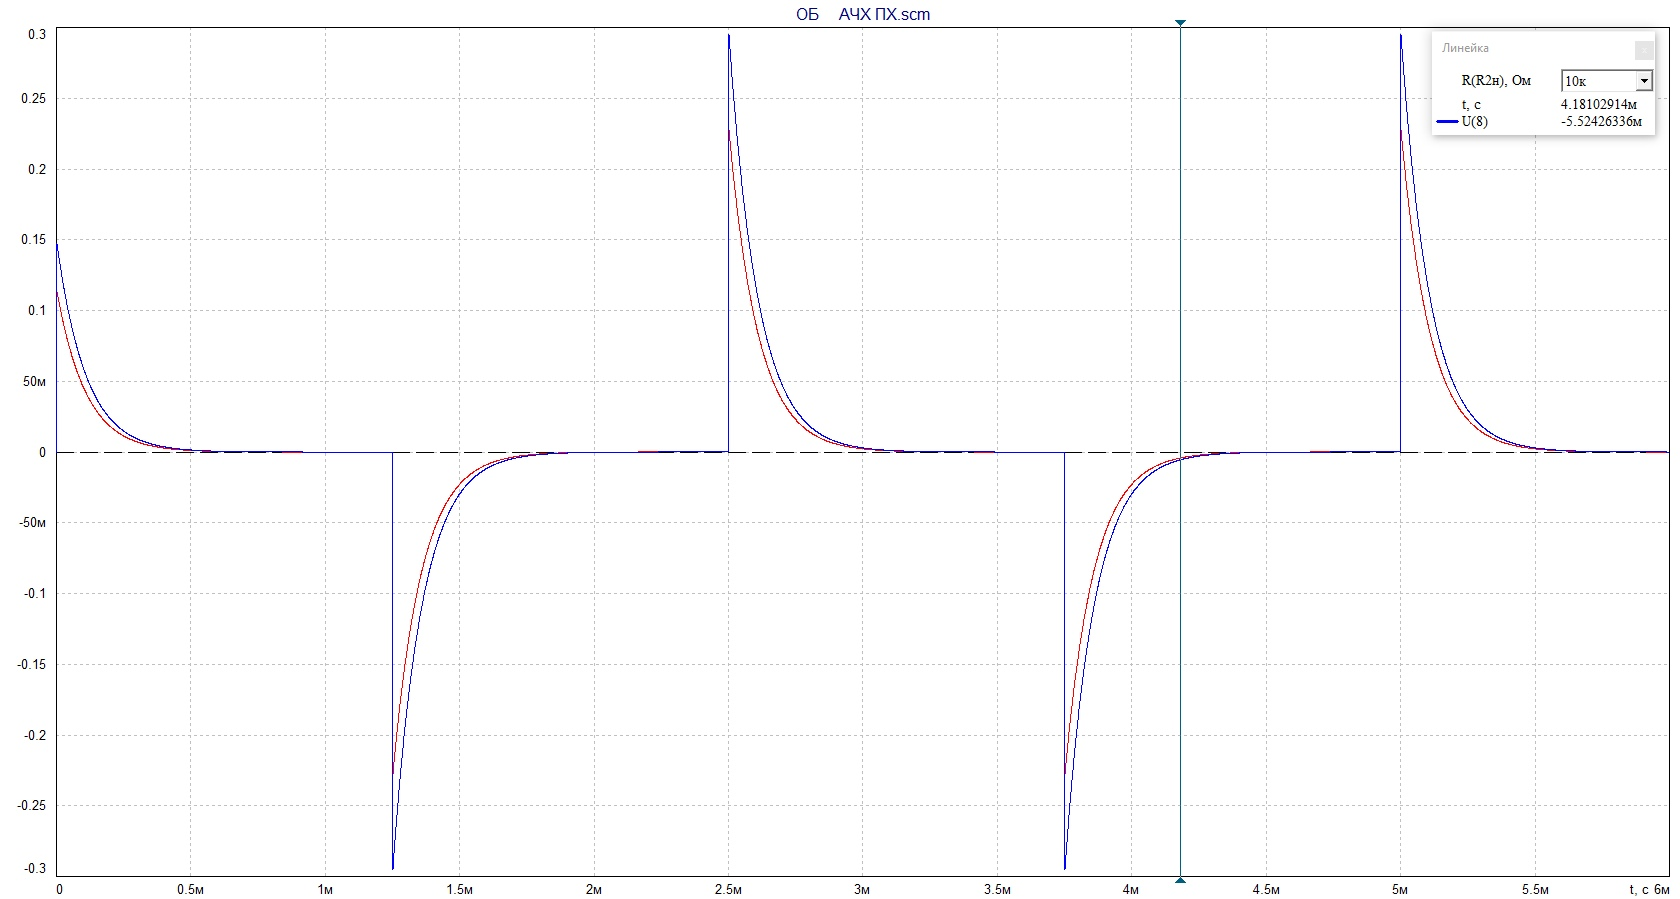
\includegraphics[scale=0.28]{5.4.jpg}
    \end{center}

    ПХ при $R_1$ = 10О Ом, f = 400 Гц

    \begin{center}
        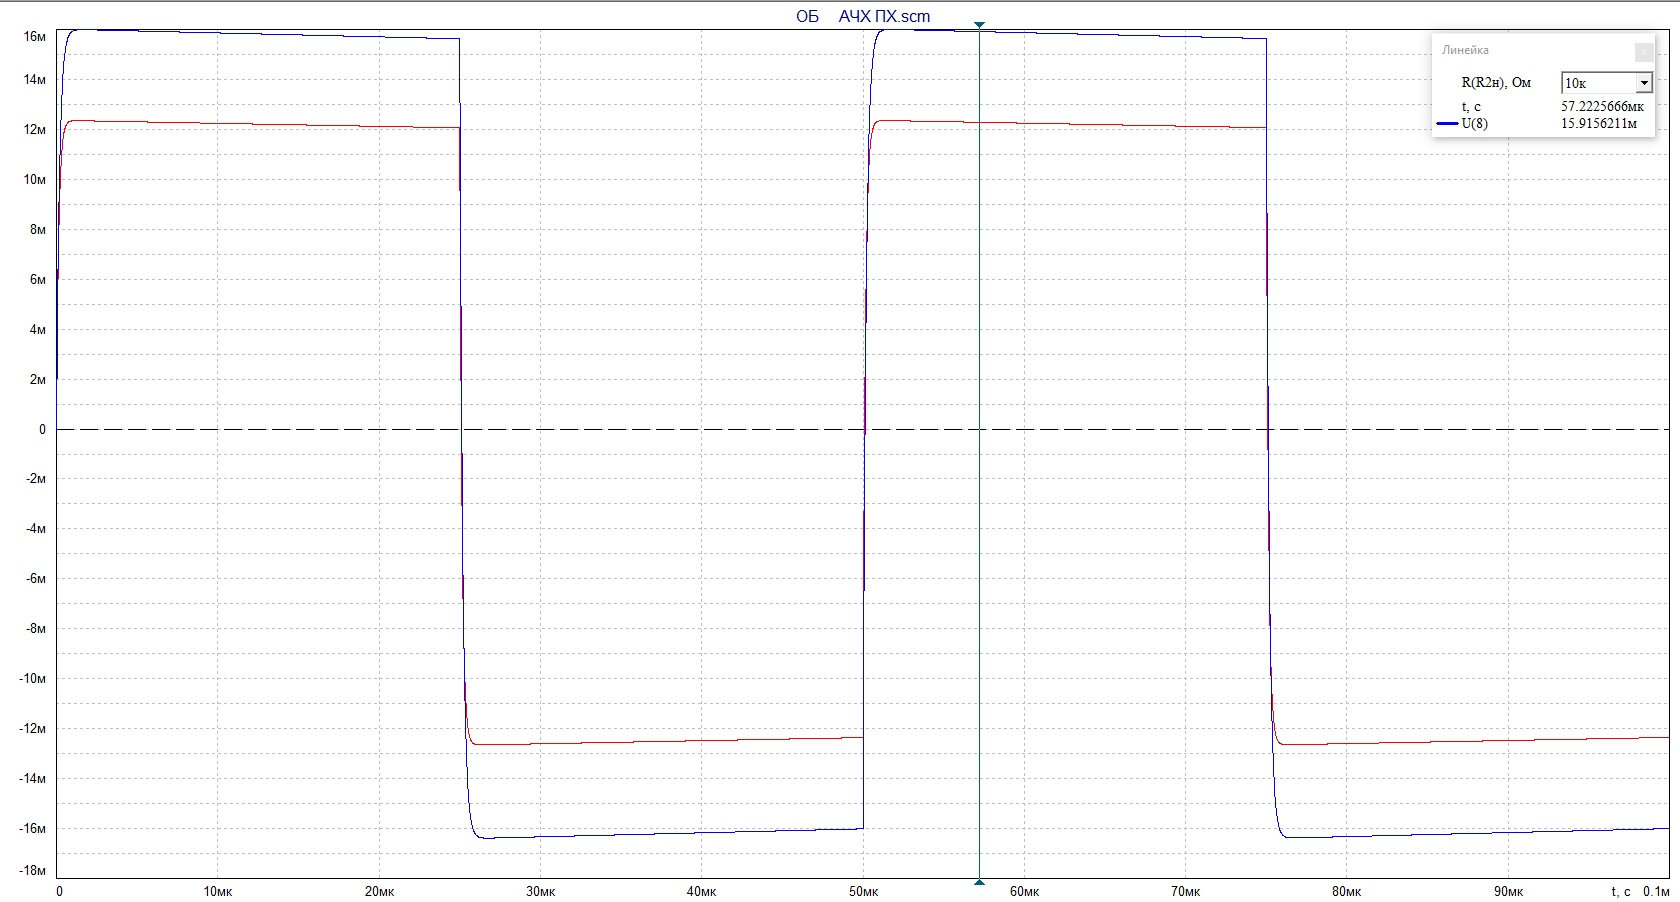
\includegraphics[scale=0.28]{5.5.jpg}
    \end{center}
    
    ПХ при f = 20 кГц, $R_1$ = 1000 Ом 

    \begin{table}[ht]
        \small
        \begin{center}
            \begin{tabular}{|c|c|c|c|c|c|}
                \hline
                № & $C_{p1}$ & $K_{\text{скв}}$ & $f_{\text{н}}$ & $f_{\text{в}}$ & \parbox[c][1.5cm]{3cm}{\begin{center}∆ \\при $t_{\text{и}}$= 1.25 мс \end{center}}
                \tabularnewline
                \hline
                п/п & мкФ & дБ & Гц & МГц & \%
                \tabularnewline
                \hline
                1 & 1 & 1.841 & 158 & 1.1 & 71.20 
                \tabularnewline
                \hline
                2 & 10 & 1.841 & 15.8 & 1.1 & 12.05
                \tabularnewline
                \hline
            \end{tabular}
        \end{center}
    \end{table}

    \begin{center}
        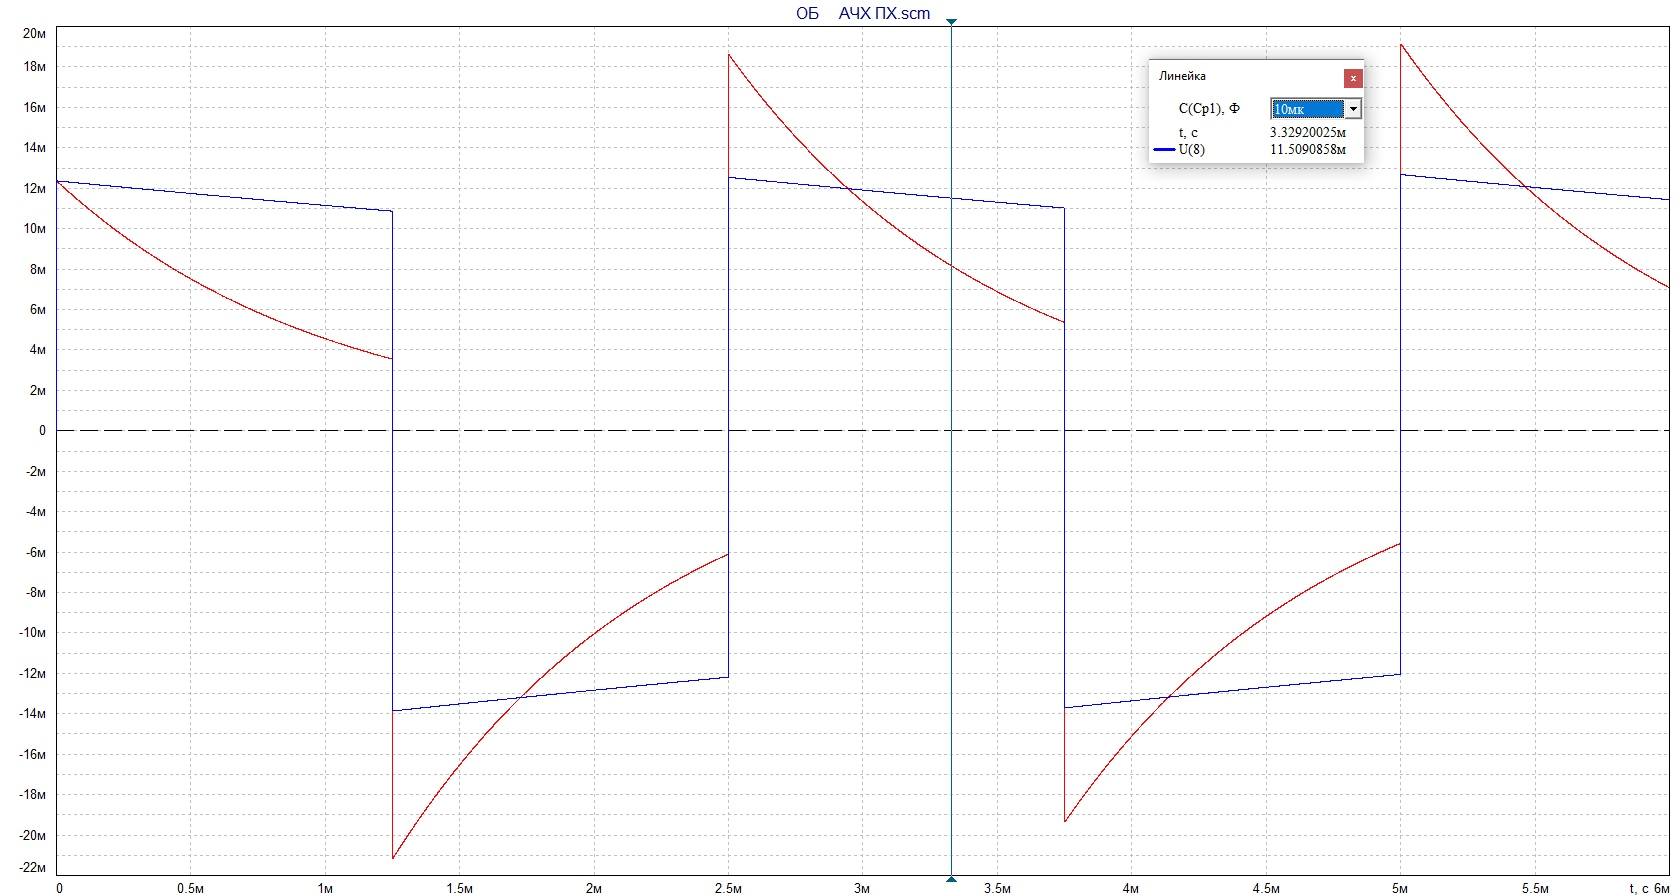
\includegraphics[scale=0.3]{5.6.jpg}
    \end{center}
    ПХ для различных $C_{r1}$

    \begin{center}
        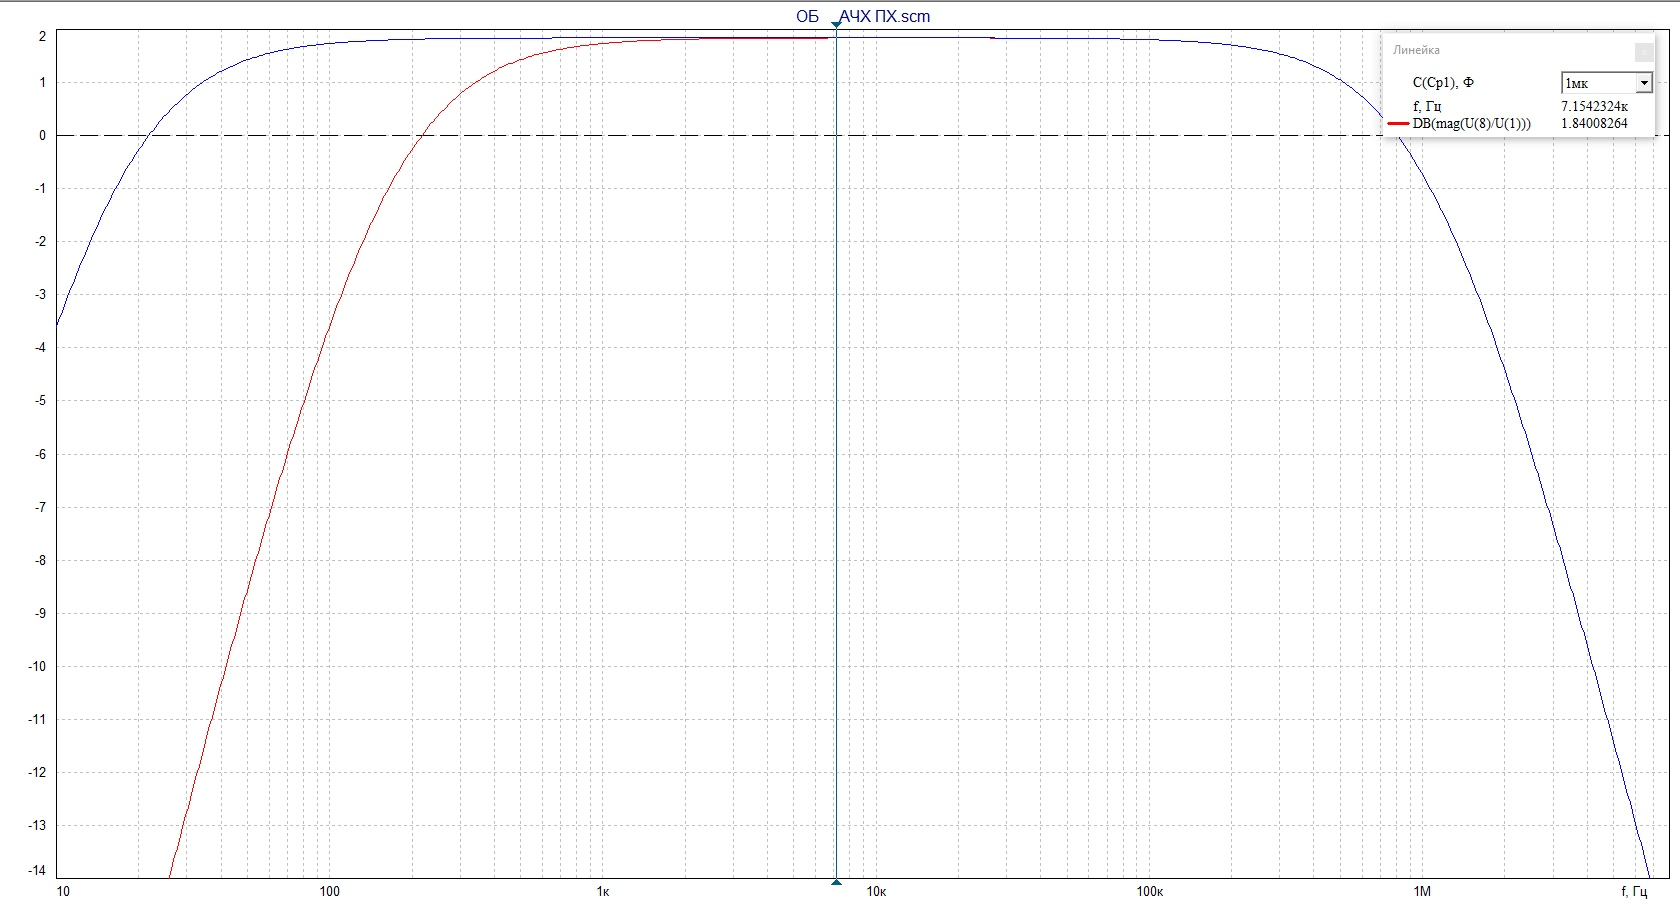
\includegraphics[scale=0.3]{5.7.jpg}
    \end{center}
    АЧХ для различных $C_{r1}$

    \textbf{Выводы по пункту 5:}
    \vspace{-6ex}
    \begin{singlespace}
        \begin{itemize}
            \item Изменение сквозного коэффициента усиления прямо пропорционально изменению $R_2$ и обратно пропорционально изменению $R_1$.
            \item Изменение частоты $f_{\text{н}}$ зависит от изменения $R_1$, а изменение частоты $f_{\text{в}}$ зависит от изменения $R_2$. При этом данная зависимость имеет обратную пропорциональность.
            \item Изменение спада вершины импульса обратно пропорционально изменению $R_1$.
            \item Изменение времени нарастания импульса прямо пропорционально изменению $R_2$.
            \item Изменение частоты $f_{\text{н}}$ обратно пропорционально изменению $C_{p1}$.
            \item Изменение спада вершины импульса обратно пропорционально изменению $C_{p1}$.
        \end{itemize}
    \end{singlespace}
\end{document}